\begin{tikzpicture}[
    inputnode/.style={rectangle, double, draw=red!75, fill=red!50, very thick, minimum size=7mm, inner sep=8pt, rounded corners=1mm},
    outputnode/.style={rectangle, double, draw=black!60, thick, minimum size=7mm, inner sep=8pt, rounded corners=1mm},
    modulenode/.style={rectangle, draw=ForestGreen!60, very thick, minimum size=7mm, inner sep=8pt, rounded corners=1mm},
    algonode/.style={rectangle, draw=black!60, fill=cyan!2.5, thick, minimum size=7mm, inner sep=6pt, font=\ttfamily\scriptsize},
    cheatnode/.style={rectangle, fill=purple!65, minimum height=7mm, inner sep=3pt, rounded corners=1mm, font=\ttfamily\scriptsize},
    algonote/.style={black, rotate=-90, font=\footnotesize},
    noarrownormal/.style={black!75, very thick, rounded corners=5pt},
    arrownormal/.style={noarrownormal, arrows={-Latex[fill=white]}},
    algonodelinks/.style={cyan!25!white, thick},
    scale=0.35
]

\def\legendtopx{-8}
\def\legendtopy{2}

\small\sffamily

\node[inputnode] (hits) {\begin{minipage}{4cm}
    \centering
    \color{white}
    \bfseries Processed hits
    \vspace{1em}
    {
\includegraphics[width=4cm, trim={0 0 14cm 0}, clip]{pandora/figure_Pandora/hits_white.pdf}}
\end{minipage}};

{
    \footnotesize
    \draw[Latex-Latex, white] 
            (-1cm,-2.975cm) node [right] {$x$, drift direction} -| 
            (-2cm,-1.975cm) node [right, rotate=90] {$w$, wire position}; 
    
    \draw[Latex-Latex] 
            (17.2cm+1cm,-3.3cm) node [right] {$x$, drift direction} -| 
            (17.2cm,    -3.3cm+1cm) node [right, rotate=90] {$w$, wire position}; 
}

%%%%%%%%%%%% ----------------- PandoraFastReco ----------------- %%%%%%%%%%%%
\begin{scope}[local bounding box=frBB]
    \node[modulenode] (fastreco) [right=0.5cm of hits] {
        \begin{minipage}{1.65cm}
            \centering
            \bfseries Pandora FastReco
        \end{minipage}};
\end{scope}
%%%%%%%%%%%% ----------------- PandoraFastReco ----------------- %%%%%%%%%%%%

%%%%%%%%%%%% ----------------- PandoraCosmicRemoval----------------- %%%%%%%%%%%%
\begin{scope}[local bounding box=cRemovlBB]
    \node[modulenode] (masterRemoval) [right=0.5cm of fastreco] {
        \begin{minipage}{2cm}
            \centering
            Removing \emph{unambiguous} cosmic(s)
        \end{minipage}
    };
\end{scope}
%%%%%%%%%%%% ----------------- PandoraCosmicRemoval----------------- %%%%%%%%%%%%

%%%%%%%%%%%% ----------------- PandoraSliceID ----------------- %%%%%%%%%%%%
\node[modulenode, minimum size=1mm, inner sep=0pt] (slcID) [right=of masterRemoval] {};
%%%%%%%%%%%% ----------------- PandoraSliceID ----------------- %%%%%%%%%%%%


%%%%%%%%%%%% ----------------- PandoraNu ----------------- %%%%%%%%%%%%
\begin{scope}[local bounding box=neutrinoBB]
    \node[modulenode] (neutrino) [below right=0.25cm and 1.5cm of slcID.center] {\begin{minipage}{1.65cm}
        \centering
        \bfseries \underline{Pandora} \underline{Neutrino}
    \end{minipage}};
\end{scope}
%%%%%%%%%%%% ----------------- PandoraNu ----------------- %%%%%%%%%%%%

%%%%%%%%%%%% ----------------- PandoraCosmic ----------------- %%%%%%%%%%%%
\begin{scope}[local bounding box=cosmicBB]
    \node[modulenode] (cosmic) [above right=0.25cm and 1.5cm of slcID.center] {\begin{minipage}{1.65cm}
        \centering
        \bfseries Pandora Cosmic
    \end{minipage}};
\end{scope}
%%%%%%%%%%%% ----------------- PandoraCosmic ----------------- %%%%%%%%%%%%

%%%%%%%%%%%% ----------------- NeutrinoID ----------------- %%%%%%%%%%%%

\begin{scope}[local bounding box=nuIDBB]
    \node[modulenode] (nuID) [right=4.5cm of slcID] {\begin{minipage}{2cm}
        \centering
        Neutrino interaction identification
    \end{minipage}};
\end{scope}
%%%%%%%%%%%% ----------------- NeutrinoID ----------------- %%%%%%%%%%%%

%%%%%%%%%%%% ----------------- CONSOLIDATED OUT ----------------- %%%%%%%%%%%%
\node (midout1) [below right=0.1cm and -1cm of masterRemoval] {};
\node[outputnode] (unambiguousCosmic) [below right=0.5cm and -1cm of midout1] {Unambiguous cosmic};
\coordinate (coordMidOut1) at (midout1);



\node[outputnode] (definiteOut) [right=0.5cm of nuID] {
    \begin{minipage}{4cm}
        \centering
        Reco. $\nu$ candidates\\+\\residual cosmics

        \vspace{1em}
        {\color{gray}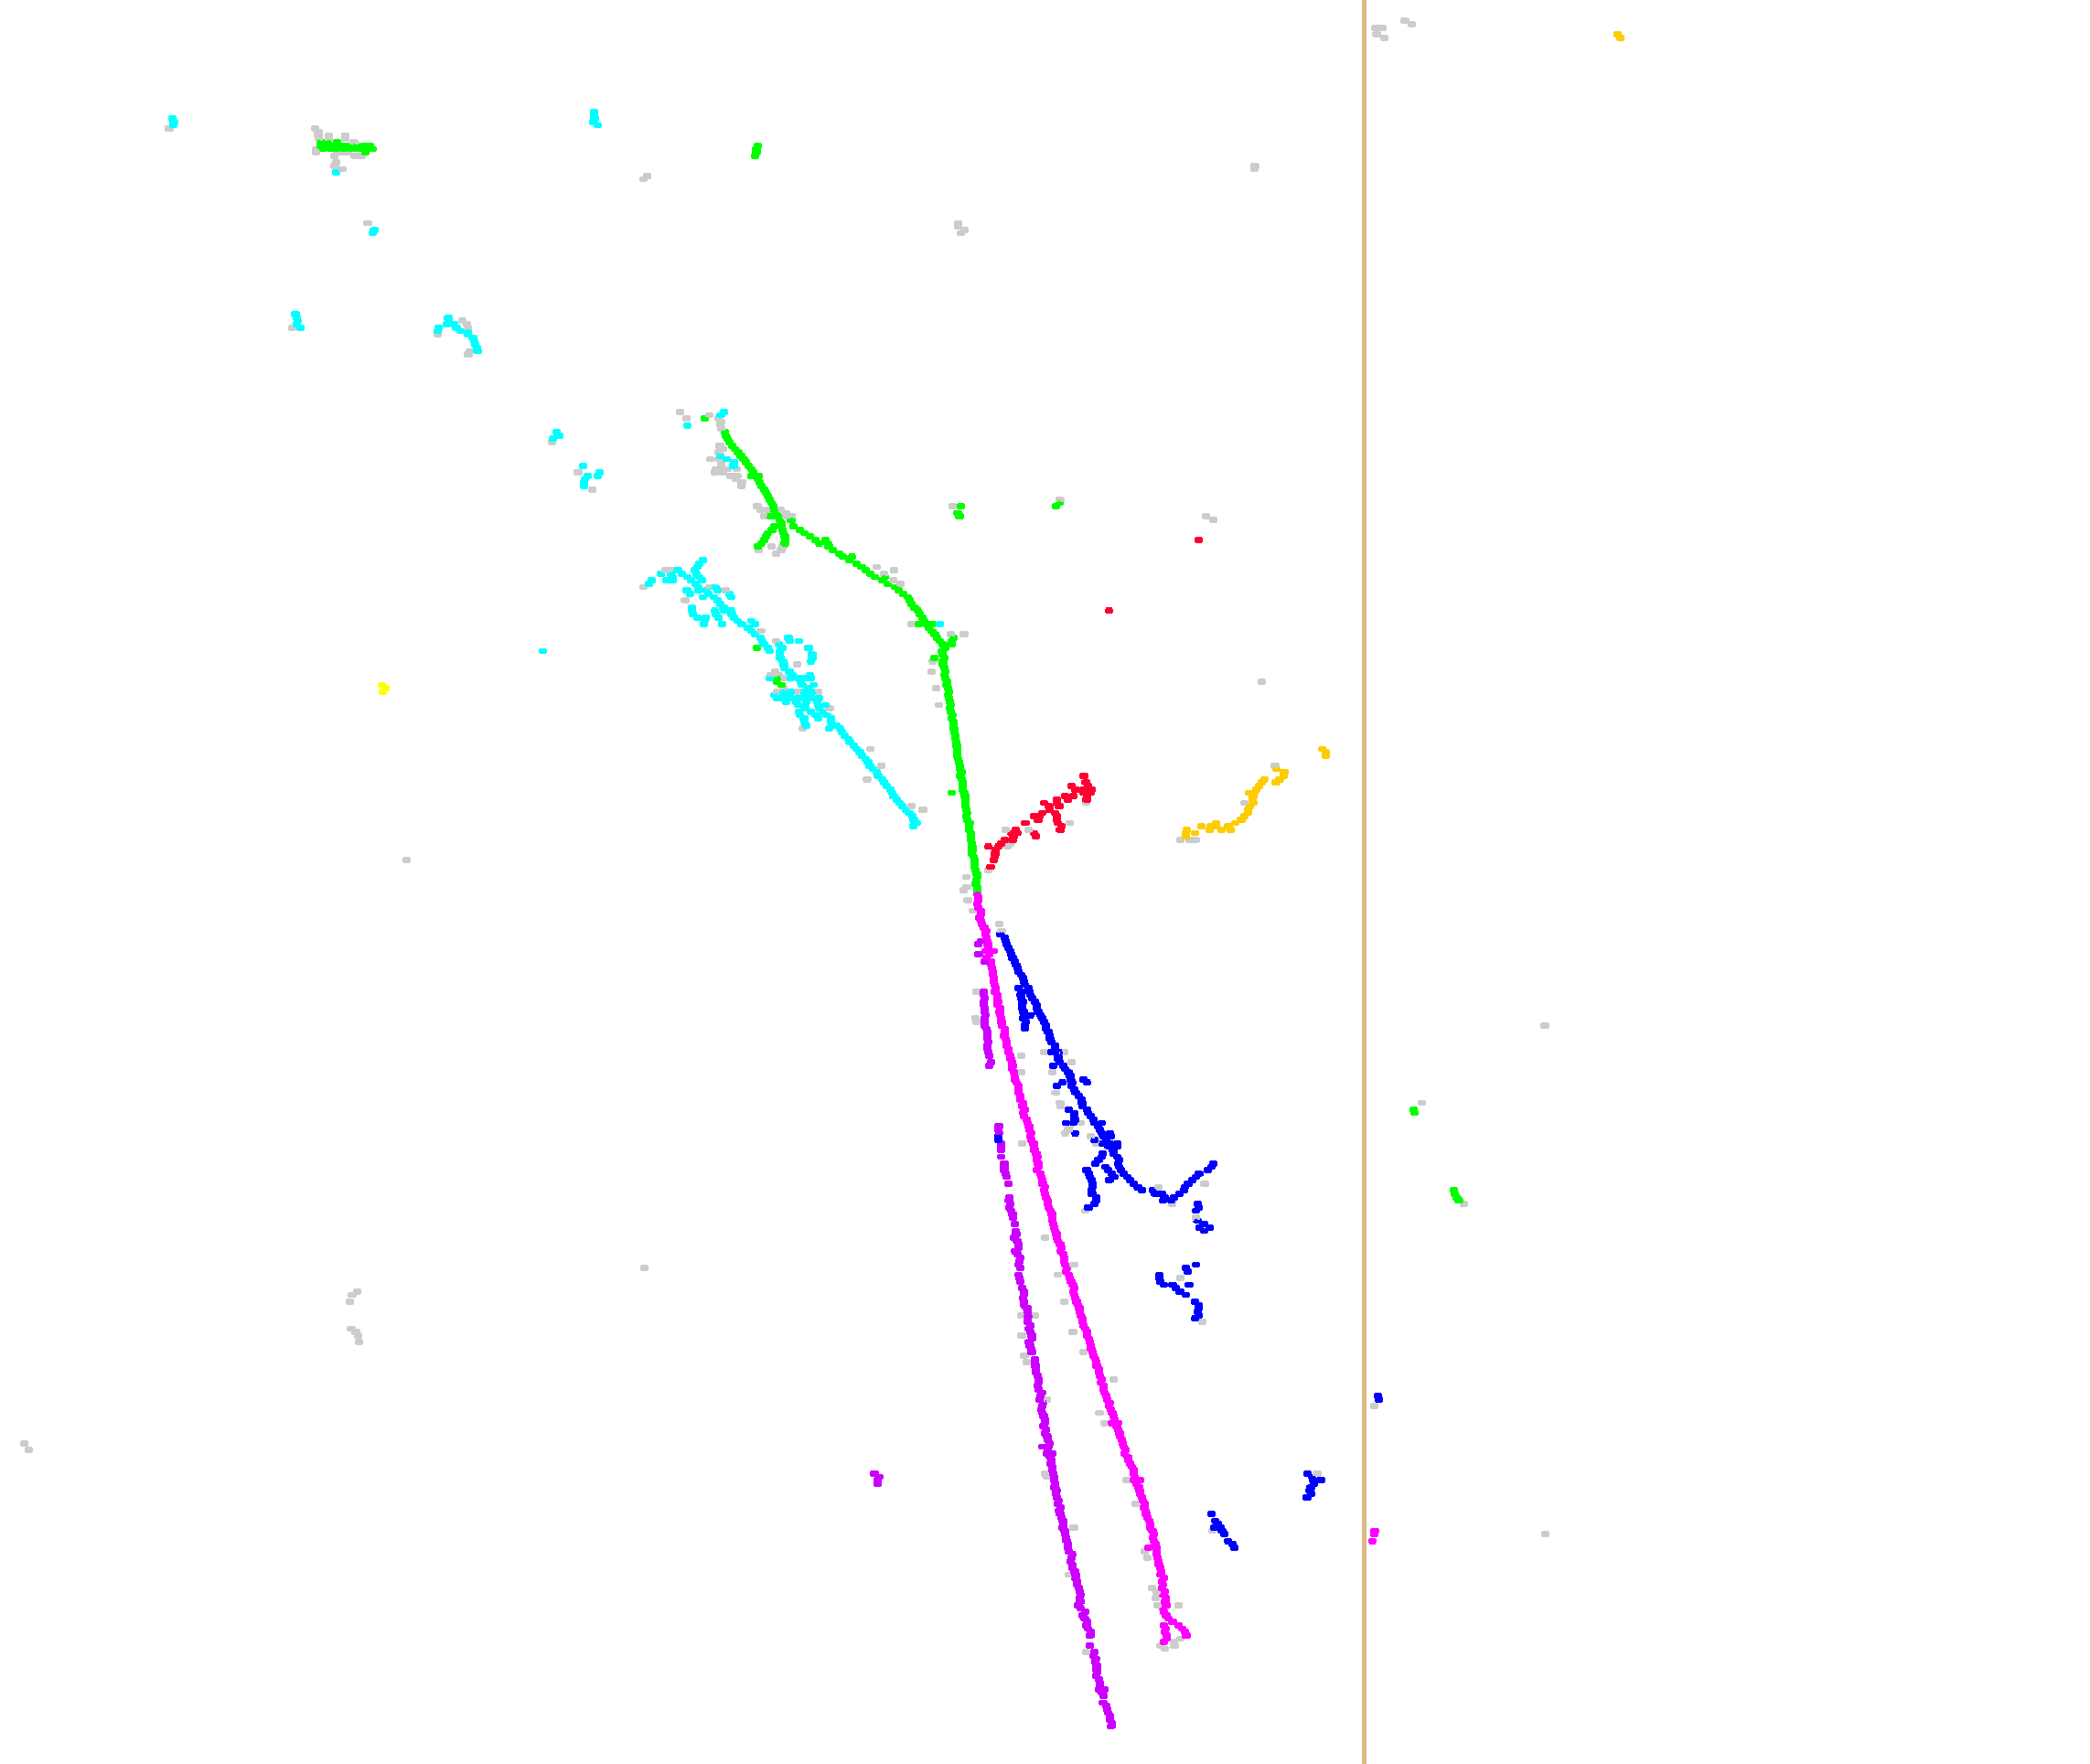
\includegraphics[width=4cm, trim={0 0 14cm 0}, clip]{pandora/figure_Pandora/cheated_cluster_2d.pdf}}
    \end{minipage}
};

%%%%%%%%%%%% ----------------- CONSOLIDATED OUT ----------------- %%%%%%%%%%%%

%%%%%%%%%%%% ----------------- ARROWS ----------------- %%%%%%%%%%%%

\draw[arrownormal, double] (hits.east) -- (fastreco.west);
\draw[arrownormal, double] (fastreco.east) -- (masterRemoval.west);
\draw[arrownormal] (masterRemoval.east) -- (slcID.west);

\draw[arrownormal] (masterRemoval.south) ++ (-2pt, 0) |- (coordMidOut1) -| (unambiguousCosmic);

\draw[arrownormal] (slcID.south) |- (neutrino.west);
\draw[arrownormal] (slcID.north) |- (cosmic.west);


\node (midout2) [left=0.5cm of nuID] {};
\coordinate (coordMidOut2) at (midout2);
\draw[noarrownormal] (neutrino.east) -| (coordMidOut2);
\draw[noarrownormal] (cosmic.east) -| (coordMidOut2);
\draw[arrownormal, double] (coordMidOut2) -- (nuIDBB.west);

% \draw[arrownormal, double] (nuIDAlgo.south) -- (definiteOut.north);
\draw[arrownormal, double] (nuID.east) -- (definiteOut.west);


%%%%%%%%%%%% ----------------- ARROWS ----------------- %%%%%%%%%%%%

\end{tikzpicture}
